\documentclass[presentation]{beamer}
\usepackage[utf8]{inputenc}
\usepackage[T1]{fontenc}
\usepackage{fixltx2e}
\usepackage{graphicx}
\usepackage{longtable}
\usepackage{float}
\usepackage{wrapfig}
\usepackage{soul}
\usepackage{textcomp}
\usepackage{marvosym}
\usepackage{wasysym}
\usepackage{latexsym}
\usepackage{amssymb}
\usepackage{hyperref}
\tolerance=1000
\providecommand{\alert}[1]{\textbf{#1}}
\usepackage{pslatex}
\usepackage{listings}
  \lstset{
    language=Python,%
    % --- basic appearance ---
    basicstyle=\ttfamily, % or \normalfont,% or \ttfamily
    columns=fullflexible,% best results for proportional fonts
    commentstyle=\normalfont\itshape\small,%
    keywordstyle=\bfseries,% or \normalfont
    %identifierstyle=\slshape,%\normalfont,%
    %procnamestyle=\scshape,%
    %procnamekeys={def},%
    % --- escaping and special displays ---
    %escapechar=|,% text between "|" will be rendered as normal TeX
    %moredelim=[il][\small\itshape]{\#},% ditto for text beween "#" and end-of-line
    %texcl,
    mathescape=true,%
    %literate={*{=}{{$\gets$ }}1 {==}{{$=$ }}1 {<=}{{$\leq$ }}1 {>=}{{$\geq$ }}1 {!=}{{$\neq$ }}1},%
    % --- display ---
    %showspaces=false,%
    showstringspaces=false,%
    %xleftmargin=2em,%
  }%
\mode<presentation>
{
  % for theme/color selection, see: http://www.hartwork.org/beamer-theme-matrix/
  \usetheme{default}
  \usecolortheme{dolphin}
  
  % no navigation bar
  \setbeamertemplate{navigation symbols}{}

  \logo{
\includegraphics[scale=0.17]{uzh-logo}}
  % To get just the UniZH coat of arms, use the following line instead:
  %\logo{
\includegraphics[scale=0.25,viewport=0 0 159 159]{uzh-logo}}

  \setlength{\parskip}{1em}
}

%% Use `\largeskip` to get a larger vertical white space between two
%% lines/paragraphs:
\newcommand{\largeskip}{\vspace{1em}}
\def\+{\largeskip}


\begin{document}

\title[GC3Pie]{%
  \textbf{GC3Pie} 
  \\ 
  A Python framework for high-throughput computing
}
\author[R.\ Murri]
{Riccardo Murri \\ \texttt{<riccardo.murri@uzh.ch>}}
\institute[GC3, Univ. of Zurich]% will appear on the bottom line
{\href{http://www.gc3.uzh.ch/}{Grid Computing Competence Centre}, 
  \href{http://www.uzh.ch/}{University of Zurich}
  \\ \url{http://www.gc3.uzh.ch/}}
\date[NG2011]{NorduGrid Conference, 2011-05-10}
\maketitle

%% turn off logo after front page
\logo{}

\begin{frame}
\frametitle{A typical high-throughput use case?}
\label{sec:1}
  Run application \emph{A} on a range of different inputs.
  Each input is a different file (or a set of files).

  Then collect output files and post-process them, e.g., gather some
  statistics.

  Typically implemented by a set of \texttt{sh} or \texttt{perl}
  scripts to drive execution on a local cluster.
\end{frame}

\begin{frame}
  \frametitle{Potential issues}
  \label{sec:2}

  \begin{enumerate}
  \item \textbf{Portability:} Cannot run on a different cluster without rewriting
    all the scripts.
  \item \textbf{Code reuse:} Scripts are often very tied to a certain purpose, so
    they are difficult to reuse.
  \item \textbf{Heavy maintenance:} the more a script does its job well, the more
    you'll find yourself adding ``generic'' features and maintaining
    requests from other users.
  \end{enumerate}
\end{frame}

\begin{frame}
  \frametitle{What is GC3Libs?}
  \label{sec:3}
  GC3Libs is a \href{http://www.python.org/}{Python} library of
  re-usable Python components to combine scientific applications into
  high-throughput workflows.

  GC3Libs features:
  \begin{itemize}
  \item drive application execution on
    \href{http://www.nordugrid.org/arc/}{ARC} and
    \href{http://www.oracle.com/us/products/tools/oracle-grid-engine-075549.html}{SGE}
    clusters,
  \item customize execution control based on application type,
  \item compose applications to form complex execution patterns.
  \end{itemize}
  
  GC3Libs is part of a larger pack of tools called \href{http://gc3pie.googlecode.com/}{GC3Pie}.
  \end{frame}

  \begin{frame}
    \frametitle{What is GC3Pie, then?}
    \label{sec:4}

    \href{http://gc3pie.googlecode.com/}{GC3Pie} consists of:
    
    \begin{itemize}
    \item \emph{GC3Libs:} re-usable Python components to drive application
      execution on Grids and clusters.
    \item \emph{GC3Utils:} simple command-line interface to the core GC3Libs
      functionality: submit/monitor/kill a job, retrieve output, etc.
    \item \emph{GC3Apps:} Driver scripts developed for specific groups, but that
      may be of independent general interest.  (E.g., running the
      \href{http://www.rosettacommons.org/manuals/archive/rosetta3.1_user_guide/app_dock.html}{Rosetta Docking} application on a large set of inputs.)
    \end{itemize}
  \end{frame}

  \begin{frame}
    \frametitle{How could this solve any issues?}
    \label{sec:5}

    \textbf{Portability:} GC3Libs aims at providing an abstraction over Grid
    and cluster resources: one single script is be able to run 
    on different computational sites.
    
    \textbf{Code reuse:} The application model, coupled with an object-oriented
    design, encourages writing more generic code that can be intergrated
    into the library.  (We hope for community-contributed code in the
    event.)
    
    \textbf{Heavy maintenance:} Generic features are part of the library. Focus
    on what makes your code special.
  \end{frame}
  
  \begin{frame}
    \frametitle{The \emph{3n+1} conjecture, a fictitious use case}
    \label{sec:7a}

    \+
    \begin{columns}[c]
      \column{0.5\linewidth}
      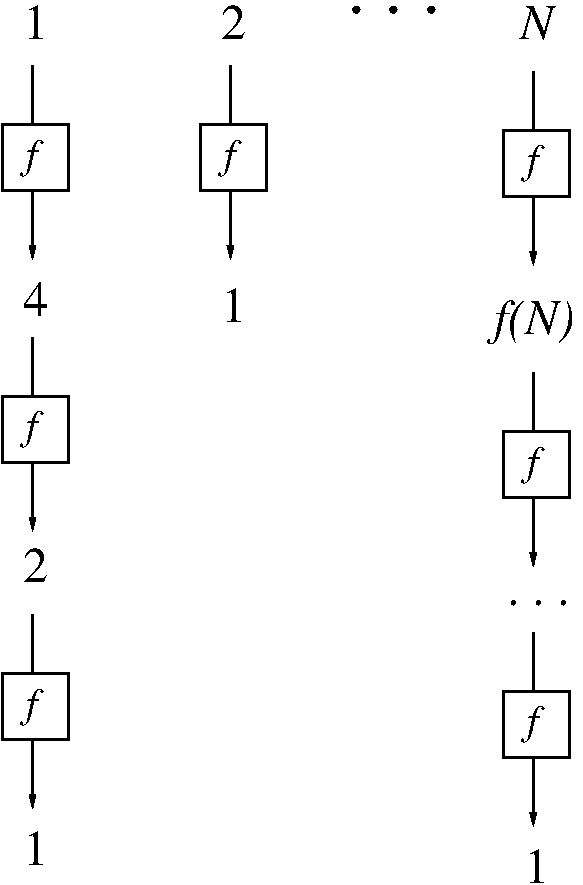
\includegraphics[height=0.8\textheight]{3n+1}
      
      \column{0.5\linewidth}
      Define a function $f$, for $n$ positive integer:
      \begin{itemize}
      \item if $n$ is even, then $f(n) = n / 2$,
      \item if $n$ is odd, then $f(n) = 3n+1$,
      \end{itemize}
      
      \+
      For every positive integer $n$, form the sequence $S(n)$:
      $n \to f(n) \to f(f(n)) \to f(f(f(n))) \to \ldots$
      
      \+
      \textbf{Conjecture:} For every positive integer $n$, the sequence $S(n)$
      eventually hits $1$.
    \end{columns}
  \end{frame}

  \begin{frame}
    \frametitle{The \emph{3n+1} conjecture on a Grid? \emph{(I)}}
    \label{sec:7}

    \+
    \begin{columns}[c]
      \column{0.5\linewidth}
      \includegraphics[height=0.8\textheight]{3n+1_A}
      
      \column{0.5\linewidth} 
      A computational job $J(n,k)$, applies
      function $f$ to the result of $J(n,k)$.
    \end{columns}
  \end{frame}

  \begin{frame}
    \frametitle{The \emph{3n+1} conjecture on a Grid? \emph{(II)}}
    \label{sec:7b}

    \+
    \begin{columns}[c]
      \column{0.5\linewidth}
      \includegraphics[height=0.8\textheight]{3n+1_S}
      
      \column{0.5\linewidth} 
      A sequence $H(n)$ of jobs computes the chain $n \to f(n) \to
      ... \to 1$.
    \end{columns}
  \end{frame}

  \begin{frame}
    \frametitle{The \emph{3n+1} conjecture on a Grid? \emph{(III)}}
    \label{sec:7c}

    \+
    \begin{columns}[c]
      \column{0.5\linewidth}
      \includegraphics[height=0.8\textheight]{3n+1_P}
      
      \column{0.5\linewidth} 
      Run one sequence $H(n)$ per each $n = 1, \ldots, N$.

      \+
      The can all run in \textbf{parallel}.
    \end{columns}
  \end{frame}

  \begin{frame}
    \frametitle{GC3Libs application model}
    \label{sec:9}

    An application is a subclass of the \texttt{gc3libs.Application} class.

    Generic \texttt{Application} class patterned after \href{http://www.nordugrid.org/documents/xrsl.pdf}{ARC's xRSL} model.

    At a minimum: provide application-specific command-line invocation.

    Advanced users can customize pre- and post-processing, react on
    state transitions, set computational requirements based on input
    files, influence scheduling.  (This is standard OOP: subclass and
    override a method.)
\end{frame}

\begin{frame}
  \frametitle{Supported applications (as of May 2011)}
  
  As of May 2011, GC3Libs has support for the following applications
  in the library core:
  \begin{itemize}
  \item \href{http://www.msg.ameslab.gov/gamess/}{GAMESS(US)}; 60K
    jobs in 2011.
  \item \href{http://www.rosettacommons.org}{Rosetta}
    (\texttt{minirosetta} and \texttt{docking{\_}protocol}); 110K jobs
    run in 2011 alone!
  \item \href{http://www.turbomole.com/}{TURBOMOLE}
  \end{itemize}
  \ldots plus a few user-developed codes.

\end{frame}

\begin{frame}[fragile]
\frametitle{The \emph{3n+1} conjecture (IV)}
\label{sec:10}

\begin{columns}
  \column{0.3\linewidth}
  \begin{center}
    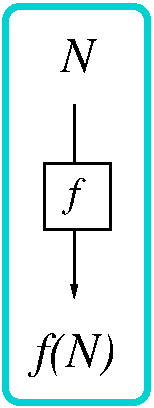
\includegraphics[height=0.8\textheight]{A}
  \end{center}

  \column{0.7\linewidth}
  Let's define the simple application that computes~$f$:
\begin{lstlisting}
class HotpoApplication(Application):
  def __init__(self, n):
    Application.__init__(
      self,
      executable = '/usr/bin/expr',
      arguments = (
          # run `expr n / 2` if n is even
          [n, '/', n] if n % 2 == 0
          # run `expr 1 + 3 * n` if n is odd
          else [1, '+', 3, '*', n]),
      stdout = "stdout.txt",
    )
\end{lstlisting}
  \end{columns}
\end{frame}

\begin{frame}
\frametitle{Composition of tasks (I)}
\label{sec:11}

  The unit of job composition is called a \texttt{Task} in GC3Libs.

  An \texttt{Application} is the primary instance of a \texttt{Task}.

  However, a single task can be composed of many applications.
  A task is a composite object: tasks can be composed of other tasks.

  Workflows are built by composing tasks in different ways.
  A ``workflow'' is a task, too.
\end{frame}
\begin{frame}
\frametitle{Composition of tasks (II)}
\label{sec:12}

  The \texttt{SequentialTask} class takes a list of jobs and executes them
  one after the other. Subclass and override the \texttt{next()} method to
  determine early exit conditions, or to modify the list dynamically.

  The \texttt{ParallelTask} class takes a list of jobs and executes all of
  them in parallel.  It's done when all jobs are done: there's an
  implicit synchronization barrier at the end.
  
\end{frame}

\begin{frame}[fragile]
\frametitle{The \emph{3n+1} conjecture (V)}
\label{sec:14}

\begin{columns}
  \column{0.2\linewidth}
  \begin{center}
    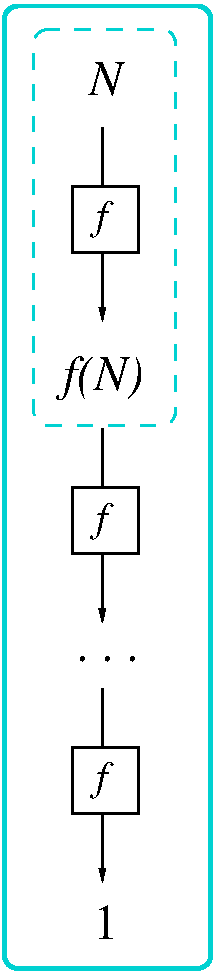
\includegraphics[height=0.8\textheight]{S}
  \end{center}

  \column{0.8\linewidth} 
  Now string together applications to compute a
  single sequence:
\begin{lstlisting}
class HotpoSequence(SequentialTask):

  def __init__(self, n):
    # compute first iteration of $f$
    self.tasks = [ HotpoApplication(n) ]
    SequentialTask.__init__(self, self.tasks)

  def next(self, k):
    last = self.tasks[k].result
    if last == 1:
      return TERMINATED
    else:
      self.tasks.append(MyApplication(last)
       return RUNNING
\end{lstlisting}
  \end{columns}
\end{frame}

\begin{frame}[fragile]
  \frametitle{The \emph{3n+1} conjecture (VI)}
  \label{sec:15}

  \begin{columns}
    \column{0.5\linewidth}
    \begin{center}
      \includegraphics[height=0.8\textheight]{3n+1_P}
    \end{center}

    \column{0.5\linewidth}
    Parallel tasks are independent by definition, so it's even easier to
    create a collection:
\begin{lstlisting}
tasks = 
  ParallelTaskCollection([ 
    HotpoSequence(n) 
      for n in range(1, N) ])
\end{lstlisting}
  
    We can run such a collection like any other \texttt{Task}.
  \end{columns}
\end{frame}

\begin{frame}
  \frametitle{A simple high-throughput script structure}
  \label{sec:16}
  
  \begin{enumerate}
  \item Get access to the Grid (e.g., authentication step)
  \item Prepare files for submission
  \item Submit jobs and monitor their status (loop)
  \item Retrieve results
  \item Postprocess and display
  \end{enumerate}
\end{frame}

\begin{frame}
\frametitle{The \texttt{Engine} class}
\label{sec:20}

  Implements core operations on applications, with \emph{non-blocking}
  semantics.

  The \texttt{progress()} method will advance jobs through their lifecycle; 
  use state-transition methods to take application-specific actions.
  (E.g., post-process output data.)
  
  An engine can automatically persist the jobs, if you so wish.
  (Just pass it a \texttt{Store} instance at construction time.)
\end{frame}

\begin{frame}
  \frametitle{How do I manage authentication with GC3Libs?}
  \label{sec:18}
  
  You don't.
  
  \emph{GC3Libs will check that there is always a valid proxy and
    certificate when attempting Grid operations, and if necessary, renew
    it.}
\end{frame}

\begin{frame}
  \frametitle{A high-throughput script, revisited with GC3Libs}
  \label{sec:21}

  \begin{enumerate}
  \item Create a gc3libs.core.Engine instance and load saved jobs into it
  \item \textbf{Create \emph{new} instance(s) of the application class}
  \item Let engine manage jobs until all are done
  \item \st{Retrieve results} (the \texttt{Engine} does it)
  \item \textbf{Postprocess and display}
  \end{enumerate}
  
  You only need to implement 2. and 5.; the rest is done by the
  \texttt{SessionBasedScript} class.
\end{frame}

\begin{frame}
\frametitle{How is GC3Libs different? (I)}
\label{sec:22}

  GC3Libs runs specific \textbf{applications}, not generic jobs.

  That is, GC3Libs exposes \texttt{Application} classes whose programming
  interface is adapted to the specific task/computation a scientific
  application performs.

  GC3Libs supports a few applications in the main library.  (Our goal
  is to support more and more.)

  You can add your own applications.  You \emph{have to} add you own
  applications. 
\end{frame}

\begin{frame}
\frametitle{How is GC3Libs different? (II)}
\label{sec:23}

  GC3Libs can run applications in parallel, or sequentially, or any
  combination of the two, and do arbitrary processing of data in the
  middle.

  Think of
  \href{http://en.wikipedia.org/wiki/Scientific_workflow_system}{workflows},
  except you can write them in the Python programming language.

  Which means, you can create them dynamically at runtime, adapting
  the schema to your problem.
\end{frame}

\begin{frame}
  \frametitle{Any questions?}
  \label{sec:24}
  
  \begin{center}
    GC3Pie home page: \href{http://gc3pie.googlecode.com}{http://gc3pie.googlecode.com}
    
    Source code: \texttt{svn co http://gc3pie.googlecode.com/svn}
    
    Mailing list: \href{mailto:gc3pie@googlegroups.com}{gc3pie@googlegroups.com}
    
    \+
    \textbf{Thank you!}
  \end{center}
\end{frame}

\end{document}
